% Provenance (never printed): see sources/outline_sources.md (Year 3: Gibbs
% energy and the phase rule in rocks, chemical potential recalled from the
% chemistry book; ternary diagrams; pseudosections, principle). Brief:
% sources/book5/BRIEFS.md, ch. 11. Curves from figdata/bachelor-3/
% gasp_tables.py, schreinemakers.py and regular_solution.py. Exercise and
% problem values in the Book 5 scratch calculator calc/ch11.py.
\chapter{चट्टानों की ऊष्मागतिकी}\label{ch:b3:petrological-thermodynamics}

कुछ मिलीमीटर चौड़ा एक गार्नेट क्षेत्र-दर-क्षेत्र बढ़ा, जब उसका शिस्ट दफ़न हुआ
और गरम हुआ। उसका बाहरी किनारा आज भी अपने कैल्सियम, लोहे और मैग्नीशियम में
उसके आसपास के बायोटाइट और प्लैजियोक्लेज़ के साथ अंतिम बार प्राप्त साम्यावस्था दर्ज रखता है।
पुस्तक 4 (स्नातक वर्ष 2) ने ऐसे संघटनों को दो अंशांकित समीकरणों से एक तापमान और एक दाब में बदला।
यह अध्याय वह बक्सा खोलता है: समीकरण कहाँ से आते हैं,
और मापी गई एन्थैल्पी व एन्ट्रॉपी की सारणियों पर कितना भरोसा किया जा सकता है,
एक चट्टान में कितने खनिज रह सकते हैं, ठोस विलयन कैसे मिलते और अलग होते हैं,
और कंप्यूटर किसी स्थूल संघटन को उन खनिज-समुच्चयों के मानचित्र में कैसे बदलता है,
जिन्हें उसे दिखाना चाहिए।

\begin{recall}
गिब्स ऊर्जा, रासायनिक विभव, सक्रियता और साम्य स्थिरांक,
विचरण और प्रावस्था नियम, मिश्रणीयता अंतराल और लीवर नियम,
रसायन की पुस्तकों के विश्वविद्यालय-स्तरीय खंडों में हैं। एकचरी अभिक्रिया, उसकी
क्लेपेरॉन ढलान $\Delta_rS/\Delta_rV$, निश्चर बिंदु और
सारणियों से परिकलित ऐलुमिनोसिलिकेट आरेख पुस्तक 4 (स्नातक वर्ष 2) में हैं, उसके
कायांतरी संलक्षणी वाले अध्याय में; भूतापमापी और भूदाबमापी,
गार्नेट--बायोटाइट विनिमय तापमापी और GASP दाबमापी, P--T--t पथों वाले अध्याय में;
त्रिकोणीय आरेख और कोटेक्टिक, मैग्मा वाले अध्याय में। एक ठोस
विलयन और उसके अंत्य-सदस्य पुस्तक 3 (स्नातक वर्ष 1) में हैं, खनिजों वाले
अध्याय में।
\end{recall}

\section{सारणियों से साम्य}\label{sec:b3:petrological-thermodynamics:tables}

स्थिर संघटन वाले खनिजों के बीच किसी अभिक्रिया के लिए तापमान
$T$ और दाब $P$ पर साम्य $\Delta_rG(T, P) = 0$ होता है। सारणियाँ
\qty{298.15}{K} और \qty{1}{bar} पर प्रत्येक खनिज की निर्माण-एन्थैल्पी, एन्ट्रॉपी
और मोलर आयतन, तथा तापमान-निर्भर ऊष्माधारिता $C_p(T)$ देती हैं।
पुस्तक 4 (स्नातक वर्ष 2) ने $\Delta_rH$, $\Delta_rS$ और $\Delta_rV$ को स्थिरांक माना था।
सामान्य परिणाम निम्नलिखित है।

\begin{theorem}[तापमान $T$ और दाब $P$ पर अभिक्रिया की गिब्स ऊर्जा]\label{thm:b3:petrological-thermodynamics:dg}
मान लीजिए एक अभिक्रिया के लिए, $T_0 = \qty{298.15}{K}$ और \qty{1}{bar} पर,
एन्थैल्पी $\Delta_rH^\circ$ और एन्ट्रॉपी $\Delta_rS^\circ$, ऊष्माधारिता
परिवर्तन $\Delta_rC_p(T)$ और ठोसों के बीच आयतन-परिवर्तन $\Delta_rV$,
जो $T$ और $P$ से स्वतंत्र हो। तब
\[
  \Delta_rG(T, P) = \Delta_rH^\circ + \int_{T_0}^{T}\Delta_rC_p\,\mathrm dT
  - T\Bigl(\Delta_rS^\circ + \int_{T_0}^{T}\frac{\Delta_rC_p}{T}\,\mathrm dT\Bigr)
  + (P - 1)\,\Delta_rV ,
\]
और साम्य रेखा है $P = 1 - \Delta_rG(T, 1)/\Delta_rV$।
\end{theorem}

\begin{proof}
\qty{1}{bar} पर $(\partial\Delta_rH/\partial T)_P = \Delta_rC_p$ और
$(\partial\Delta_rS/\partial T)_P = \Delta_rC_p/T$; $T_0$ से समाकलन करने पर
$\Delta_rH(T)$ और $\Delta_rS(T)$ मिलते हैं, और $\Delta_rG = \Delta_rH -
T\Delta_rS$। स्थिर $T$ पर, $(\partial\Delta_rG/\partial P)_T = \Delta_rV$,
परिकल्पना के अनुसार स्थिर है; 1 से $P$ तक समाकलन $(P - 1)\Delta_rV$ जोड़ता है।
$\Delta_rG(T, P) = 0$ रखने पर रेखा प्राप्त होती है।
\end{proof}

दोनों समाकल आंशिक रूप से एक-दूसरे को निरस्त करते हैं: उनका योग है $\int_{T_0}^T\Delta_rC_p(1 -
T/T')\,\mathrm dT'$ है, जिसमें गुणक $1 - T/T'$ ऋणात्मक और छोटा है,
जहाँ $T'$ का मान $T$ के निकट है। ठोसों के बीच $\Delta_rC_p$ स्वयं छोटा होता है,
क्योंकि किसी खनिज की ऊष्माधारिता लगभग उसके ऑक्साइडों की ऊष्माधारिताओं के
योग के बराबर होती है। इसलिए स्थिर-गुण सन्निकटन अच्छा है, और सारणियाँ
बताती हैं कि यह कितना अच्छा है। GASP अभिक्रिया के लिए,
\[
  \ce{3 CaAl2Si2O8 <=> Ca3Al2Si3O12 + 2 Al2SiO5 + SiO2},
\]
सारांश सारणी देती है $\Delta_rH^\circ = \qty{-36.3}{kJ}$,
$\Delta_rS^\circ = \qty{-130.7}{J.K^{-1}}$ और $\Delta_rV =
\qty{-6.61}{J.bar^{-1}}$, जिससे \qty{19.8}{bar/K} ढलान की एक रेखा मिलती है; उच्च-तापमान
सारणियाँ, जिनमें ऊष्माधारिताएँ शामिल हैं, हर \qty{100}{K} पर
$\Delta_rG$ का मान देती हैं, और दोनों रेखाएँ
\qty{1200}{K} तक \qty{0.12}{kbar} से कम भिन्न हैं (नीचे का आरेख)।
% ledger: rh95:gasp-298, rh95:gasp-ht

प्रयोग उतनी अच्छी तरह सहमत नहीं हैं। पिस्टन-सिलिंडर प्रेस में 900 से
\qty{1250}{\celsius} तक उलटाई गई यह अभिक्रिया \qty{627}{\celsius} पर सारणी-मानों से
\qty{0.9}{kbar} ऊँची निकली, और \qty{927}{\celsius} पर \qty{1.9}{kbar} ऊँची
निकली। $\Delta_rV = \qty{-6.61}{J.bar^{-1}}$ के साथ,
\qty{1.9}{kbar} का अर्थ है \qty{12.6}{kJ} की त्रुटि $\Delta_rH$ में;
चार निर्माण-एन्थैल्पियों की अनिश्चितताएँ: ग्रॉसुलर के लिए \qty{3.2}{kJ},
ऐनॉर्थाइट और काइनाइट के लिए \qty{2.0}{kJ}, और
क्वार्ट्ज़ के लिए \qty{1.0}{kJ}, मिलकर $\Delta_rH$ में लगभग \qty{8}{kJ} हो जाती हैं। कैलोरीमिति हर
खनिज को कुछ किलोजूल तक निश्चित करती है; बड़ी सूत्र-इकाइयों वाली अभिक्रिया इन त्रुटियों को गुणा करती है
और उन्हें एक छोटे आयतन-परिवर्तन से भाग देती है।
% ledger: rh95:gasp-298, kn88:gasp

\begin{definition}[आंतरिक रूप से सुसंगत ऊष्मागतिक आँकड़ा-समुच्चय]\label{def:b3:petrological-thermodynamics:dataset}
एक \emph{आंतरिक रूप से सुसंगत ऊष्मागतिक आँकड़ा-समुच्चय}\index{आंतरिक रूप से सुसंगत ऊष्मागतिक आँकड़ा-समुच्चय}
वह सारणी है जिसमें अनेक खनिजों और तरलों के मानक गुण
(निर्माण-एन्थैल्पी, एन्ट्रॉपी, आयतन, ऊष्माधारिता,
तापीय प्रसार और संपीड्यता) एक साथ समायोजित, कैलोरीमिति की अनिश्चितताओं की सीमा के भीतर,
ताकि उससे परिकलित हर साम्य
उन उलटे प्रयोगों से गुज़रे जिन पर उसका समायोजन हुआ था।
\end{definition}

ऐसा आँकड़ा-समुच्चय एक बार भारित न्यूनतम वर्ग या रैखिक प्रोग्रामन द्वारा
सभी कोष्ठकों पर एक साथ समायोजित किया जाता है, और फिर उसके खनिजों के बीच की हर
अभिक्रिया पर प्रयुक्त होता है, उन अभिक्रियाओं सहित जिनका प्रयोगशाला में कभी
अध्ययन नहीं हुआ। इसके अंक स्वतंत्र मापन नहीं हैं: एक एन्थैल्पी
को एक किलोजूल तक खिसकाया जा सकता है, ताकि वह उस अभिक्रिया से मेल खाए जिसमें वह भाग लेती है। भिन्न
आँकड़ा-समुच्चयों के मान कभी मिलाए नहीं जाने चाहिए।

\begin{omfigure}
\begin{tikzpicture}
\begin{axis}[omrecord, width=0.78\linewidth, height=0.5\linewidth,
  xlabel={तापमान (\unit{\celsius})}, ylabel={दाब (\unit{kbar})},
  xmin=400, xmax=1300, ymin=0, ymax=30, legend style={font=\scriptsize,
  at={(0.03,0.97)}, anchor=north west, legend cell align=left}]
% computed in figdata/bachelor-3/gasp_tables.py
\fill[omLithLime!60] (axis cs:900,19) rectangle (axis cs:1250,28);
\addplot[red!70!black, very thick] table[x=tc, y=p_kn88] {figdata/out/bachelor-3-gasp_tables-lines.dat};
\addlegendentry{प्रयोग (अंत्य-सदस्य)}
\addplot[omDef, thick, densely dashed] table[x=tc, y=p_const] {figdata/out/bachelor-3-gasp_tables-lines.dat};
\addlegendentry{सारणियाँ, स्थिर $\Delta_rH$, $\Delta_rS$}
\addplot[omDef, only marks, mark=*, mark size=1.8pt] table[x=tc, y=p_table] {figdata/out/bachelor-3-gasp_tables-tables.dat};
\addlegendentry{सारणियाँ, ऊष्माधारिता सहित}
\node[font=\scriptsize, align=center] at (axis cs:1075,26.3) {उलटे\\प्रयोग};
\node[font=\scriptsize] at (axis cs:560,4) {ऐनॉर्थाइट};
\node[font=\scriptsize, align=center] at (axis cs:560,17) {ग्रॉसुलर + काइनाइट\\+ क्वार्ट्ज़};
\end{axis}
\end{tikzpicture}

\par\smallskip{\small अंत्य-सदस्य GASP अभिक्रिया, 3 ऐनॉर्थाइट = ग्रॉसुलर +
2 काइनाइट + क्वार्ट्ज़, कैलोरीमितीय सारणियों से स्थिर
गुणों (बिंदीदार) और ऊष्माधारिता (बिंदुओं वाली) के साथ परिकलित, और वह रेखा जो
छायांकित परास (लाल) में किए गए उलटे प्रयोगों पर फ़िट की गई है, जिसे
\qty{900}{\celsius} से नीचे बहिर्वेशित किया गया है।}\label{fig:b3:petrological-thermodynamics:gasp}
\end{omfigure}
% ledger: rh95:gasp-298, rh95:gasp-ht, kn88:gasp

\section{चट्टानों में प्रावस्था नियम}\label{sec:b3:petrological-thermodynamics:phase-rule}

रसायन का प्रावस्था नियम विचरण $F = c - p + 2$ देता है, जो
$c$ घटकों और $p$ प्रावस्थाओं वाले तंत्र का है। चट्टान ऐसा ही एक तंत्र है, और
उसके खनिज यह दिखाते हैं कि वह दाब--तापमान तल के किस भाग में साम्यावस्था प्राप्त करती है।

\begin{proposition}[खनिजीय प्रावस्था नियम]\label{prop:b3:petrological-thermodynamics:goldschmidt}
दाब--तापमान तल के एक क्षेत्र में स्वतंत्र रूप से चुने गए दाब और तापमान पर
साम्यावस्था प्राप्त करने वाली चट्टान अधिक से अधिक उतनी ही प्रावस्थाएँ रखती है
जितने उसके घटक हैं: $p \le c$। यही
\emph{खनिजीय प्रावस्था नियम}\index{खनिजीय प्रावस्था नियम} है।
\end{proposition}

\begin{proof}
प्रावस्था नियम $F = c - p + 2$ स्वतंत्र प्रबल चर देता है। यदि
दाब और तापमान दोनों समुच्चय बदले बिना बदल सकें, तो उनमें से
दो स्वतंत्र हैं: $F \ge 2$, अतः $p \le c$। $p = c + 1$ प्रावस्थाओं वाली चट्टान
एकचरी रेखा पर होती है; $p = c + 2$ वाली चट्टान निश्चर बिंदु पर; इनमें से
कोई भी यादृच्छिक रूप से चुनी गई चट्टान के लिए संभावित नहीं है।
\end{proof}

जो चट्टान नियम तोड़ती है, वह या तो किसी अभिक्रिया रेखा पर साम्यावस्था में पहुँची होती है, जिसे
उसके गठन दिखा सकते हैं, या पूरी तरह साम्यावस्था तक कभी नहीं पहुँची: कोरोना गठन,
क्षेत्रित खनिज और अवशिष्ट कण सामान्य कारण हैं। घटक गिनना
सावधानी माँगता है। स्थिर संघटन वाली केवल एक प्रावस्था में रहने वाला घटक, जैसे
ज़िरकॉन, अपनी प्रावस्था के साथ हटाया जा सकता है; बाह्य भंडार द्वारा स्थिर किया गया घटक,
जैसे चट्टान में तरल बहने पर जल, मुक्त नहीं गिना जाता,
क्योंकि उसका रासायनिक विभव आरोपित होता है।

निश्चर बिंदु के चारों ओर एकचरी रेखाएँ यादृच्छिक रूप से नहीं काटतीं। $c$ घटकों वाले
तंत्र में बिंदु पर $c + 2$ प्रावस्थाएँ मिलती हैं, और वहाँ से $c + 2$ अभिक्रियाएँ
निकलती हैं, प्रत्येक $c + 1$ प्रावस्थाओं के बीच लिखी जाती है और
उस प्रावस्था के नाम पर, कोष्ठक में, नामित होती है, जिसे वह छोड़ती है।

\begin{definition}[श्राइनमेकर्स विश्लेषण]\label{def:b3:petrological-thermodynamics:schreinemakers}
\emph{श्राइनमेकर्स विश्लेषण}\index{श्राइनमेकर्स विश्लेषण} वह विधि है
जो केवल प्रावस्थाओं के संघटन से, उनके ऊष्मागतिक गुणों के किसी मापन से पहले,
निश्चर बिंदु के चारों ओर एकचरी रेखाओं को व्यवस्थित करती है: वह
रेखाओं का क्रम, प्रत्येक रेखा की स्थायी ओर, और
उनके बीच के प्रत्येक खंड के समुच्चय तय करती है।
\end{definition}

\begin{method}[श्राइनमेकर्स के नियम]\label{met:b3:petrological-thermodynamics:schreinemakers}
(1) $c + 2$ अभिक्रियाएँ लिखिए, प्रत्येक में एक प्रावस्था छोड़कर। (2) प्रत्येक रेखा
बिंदु के एक ओर स्थायी और दूसरी ओर उपस्थायी होती है।
(3) ($i$) रेखा का उपस्थायी विस्तार, जो प्रावस्था $i$ छोड़ती है, एक ऐसे खंड में
स्थित होता है जहाँ $i$ स्थायी है। (4) दो क्रमागत स्थायी रेखाओं के बीच कोई खंड
\ang{180} से अधिक नहीं फैलता। (5) किसी रेखा के आर-पार, उसके दोनों ओर के समुच्चय
उसकी अभिक्रिया के दोनों पक्षों के समुच्चय होते हैं। आँकड़ों से एक रेखा तय करने पर
पूरा गुच्छा तय हो जाता है, दर्पण-प्रतिबिंब के अतिरिक्त।
\end{method}

पुस्तक 4 (स्नातक वर्ष 2) का ऐलुमिनोसिलिकेट त्रिक बिंदु सबसे सरल स्थिति है,
जिसमें $c = 1$ और तीन रेखाएँ हैं। नीचे का आरेख एक द्वि-घटक स्थिति दिखाता है, जिसे
हर बिंदु पर \omterm{def:b3:petrological-thermodynamics:minimisation}{गिब्स ऊर्जा न्यूनीकरण} से परिकलित किया गया है।

\begin{omfigure}
\begin{tikzpicture}
\begin{axis}[omrecord, width=0.62\linewidth, height=0.5\linewidth,
  xlabel={तापमान (\unit{\celsius})}, ylabel={दाब (\unit{kbar})},
  xmin=400, xmax=800, ymin=1, ymax=9, grid=none]
% computed in figdata/bachelor-3/schreinemakers.py
\addplot[omDef, very thick] table[x=t, y=p] {figdata/out/bachelor-3-schreinemakers-ray_A_s.dat};
\addplot[omDef, thick, densely dashed] table[x=t, y=p] {figdata/out/bachelor-3-schreinemakers-ray_A_m.dat};
\addplot[omDef, very thick] table[x=t, y=p] {figdata/out/bachelor-3-schreinemakers-ray_B_s.dat};
\addplot[omDef, thick, densely dashed] table[x=t, y=p] {figdata/out/bachelor-3-schreinemakers-ray_B_m.dat};
\addplot[omDef, very thick] table[x=t, y=p] {figdata/out/bachelor-3-schreinemakers-ray_C_s.dat};
\addplot[omDef, thick, densely dashed] table[x=t, y=p] {figdata/out/bachelor-3-schreinemakers-ray_C_m.dat};
\addplot[omDef, very thick] table[x=t, y=p] {figdata/out/bachelor-3-schreinemakers-ray_D_s.dat};
\addplot[omDef, thick, densely dashed] table[x=t, y=p] {figdata/out/bachelor-3-schreinemakers-ray_D_m.dat};
\node[font=\scriptsize, fill=white, inner sep=1pt] at (axis cs:740,7.85) {(A)};
\node[font=\scriptsize, fill=white, inner sep=1pt] at (axis cs:540,8.75) {(C)};
\node[font=\scriptsize, fill=white, inner sep=1pt] at (axis cs:540,1.6) {(B)};
\node[font=\scriptsize, fill=white, inner sep=1pt] at (axis cs:740,2.15) {(D)};
\node[font=\scriptsize, align=center] at (axis cs:592,7.7) {A + B\\B + D};
\node[font=\scriptsize, align=center] at (axis cs:450,5.0) {A + D};
\node[font=\scriptsize, align=center] at (axis cs:592,2.4) {A + C\\C + D};
\node[font=\scriptsize, align=center] at (axis cs:765,5.0) {A + B\\B + C\\C + D};
\end{axis}
\end{tikzpicture}

\par\smallskip{\small द्वि-घटक तंत्र में श्राइनमेकर्स गुच्छा, जिसमें चार प्रावस्थाएँ हैं,
जिनके संघटन A (0), B ($1/3$), C ($2/3$) और D (1) हैं। यह गुच्छा काल्पनिक गुणों के लिए
परिकलित है: स्थायी रेखाएँ ठोस, उपस्थायी विस्तार बिंदीदार,
और प्रत्येक खंड में स्थायी युग्म। (D) है A + C = 2B, (A) है B + D =
2C, (C) है 2A + D = 3B और (B) है A + 2D = 3C।}\label{fig:b3:petrological-thermodynamics:schreinemakers}
\end{omfigure}

\section{ठोस विलयन}\label{sec:b3:petrological-thermodynamics:solutions}

अधिकांश शैलनिर्माणकारी खनिज ठोस विलयन होते हैं, और उनके अंत्य-सदस्य
अभिक्रियाओं में अपनी सक्रियताओं के माध्यम से आते हैं। पुस्तक 4 ने गार्नेट में ग्रॉसुलर के लिए $a = X^3$
और प्लैजियोक्लेज़ में ऐनॉर्थाइट के लिए $a = X$ लिया था।
दोनों एक ही मॉडल की स्थितियाँ हैं।

\begin{definition}[स्थल-मिश्रण सक्रियता मॉडल]\label{def:b3:petrological-thermodynamics:site-mixing}
किसी \emph{स्थल-मिश्रण सक्रियता मॉडल}\index{स्थल-मिश्रण सक्रियता मॉडल} में, खनिज के आयन
प्रत्येक क्रिस्टलीय स्थल पर यादृच्छिक रूप से मिश्रित होते हैं, अन्य स्थलों से स्वतंत्र रूप से।
किसी अंत्य-सदस्य की आदर्श सक्रियता तब सभी स्थलों पर गुणनफल होती है, जिसमें
प्रत्येक स्थल का वह भाग जिसे वह भरता है, प्रति सूत्र इकाई ऐसे स्थलों की संख्या की घात तक उठाया जाता है:
$a_i = \prod_s X_{s,i}^{\,n_s}$।
\end{definition}

एक गार्नेट $X_3Y_2\ce{Si3O12}$ में तीन डोडेकाहेड्रल स्थल $X$ होते हैं,
जिनमें \ce{Ca}, \ce{Fe}, \ce{Mg} और \ce{Mn} रहते हैं: $a_{\text{ग्रॉसुलर}} =
X_{\text{Ca}}^3$। जिस गार्नेट में $X_{\text{Ca}} = 0.10$ है, उसमें
\qty{10}{\percent} ग्रॉसुलर होता है, फिर भी उसकी सक्रियता $10^{-3}$ है। आदर्श
मॉडल विन्यासों की गिनती करता है; वास्तविक विलयनों में अतिरिक्त ऊर्जा भी होती है,
क्योंकि विभिन्न आकार के आयन जालक में विकृति उत्पन्न करते हैं।

\begin{definition}[गिब्स ऊर्जा--संघटन आरेख]\label{def:b3:petrological-thermodynamics:gx}
एक \emph{गिब्स ऊर्जा--संघटन आरेख}\index{गिब्स ऊर्जा--संघटन आरेख}
स्थिर तापमान और दाब पर, किसी तंत्र की प्रत्येक प्रावस्था की मोलर गिब्स ऊर्जा
को उसके संघटन के विरुद्ध दर्शाता है। किसी भी स्थूल संघटन का स्थायी समुच्चय
वक्रों के निचले उत्तल खोल पर स्थित होता है: जहाँ किसी प्रावस्था का वक्र खोल पर है,
वहाँ एक ही प्रावस्था होती है; और सामान्य स्पर्शरेखा के सिरों पर दो प्रावस्थाएँ।
\end{definition}

\begin{proposition}[नियमित विलयन]\label{prop:b3:petrological-thermodynamics:regular}
एक द्विआधारी विलयन में, जिसमें प्रति सूत्र इकाई एक मिश्रण स्थल है और
अंतर्क्रिया ऊर्जा $W$ है, मिश्रण की गिब्स ऊर्जा होती है
\[
  G_{\text{मिश्र}} = RT\bigl[x\ln x + (1 - x)\ln(1 - x)\bigr] + Wx(1 - x).
\]
यदि $W > 0$ है, तो विलयन $T_c =
W/(2R)$ से ऊपर हर संघटन पर स्थायी है; $T_c$ से नीचे वक्र के दो विभक्ति बिंदु
होते हैं, और उसकी सामान्य स्पर्शरेखा के दो बिंदुओं के बीच के संघटन दो प्रावस्थाओं में बँट जाते हैं।
\end{proposition}

\begin{proof}
पहला पद यादृच्छिक मिश्रण की विन्यासी एन्ट्रॉपी का $-T$ गुना है;
दूसरा पद सबसे सरल अतिरिक्त ऊर्जा है, सममित और दोनों सिरों पर शून्य।
दो बार अवकलन करने पर $G''_{\text{मिश्र}} = RT/[x(1 - x)] - 2W$ प्राप्त होता है। $x$ पर इसका
$x = 1/2$ पर यह $4RT - 2W$ के बराबर है, जो हर $x$ के लिए, यदि $T > W/(2R)$ है, धनात्मक है।
नीचे $G''_{\text{मिश्र}} < 0$ होता है, और यह $1/2$ के आसपास के एक अंतराल पर होता है:
वहाँ वक्र नीचे की ओर मुड़ता है, वक्र के दो बिंदुओं के बीच की सीधी रेखा
उसके नीचे रहती है, और ऊपर दी गई परिभाषा के अनुसार चट्टान दो
प्रावस्थाओं वाली होती है।
\end{proof}

\begin{definition}[सॉल्वस, निर्विलयन]\label{def:b3:petrological-thermodynamics:solvus}
\emph{सॉल्वस}\index{सॉल्वस} तापमान--संघटन तल में वह वक्र है,
जो एक ठोस विलयन के मिश्रणीयता अंतराल की सीमा बनाता है: इसके नीचे, मध्यवर्ती संघटन का एक एकल क्रिस्टल
अस्थायी होता है और दो में बँट जाता है।
\emph{निर्विलयन (खनिज)}\index{निर्विलयन (खनिज)} वह विभाजन है जो शीतलन पर
क्रिस्टल के भीतर होता है: एक संघटन की पट्टिकाएँ दूसरे संघटन के पोषक में
बढ़ती हैं।
\end{definition}

क्षार फ़ेल्डस्पार, पाइरॉक्सीन और एम्फ़ीबोल में निर्विलयन पट्टिकाएँ दिखती हैं,
जो सूक्ष्मदर्शी के नीचे या आँख से दिखाई देती हैं: कई ग्रेनाइट का पर्थाइट
एक निर्विलयित क्षार फ़ेल्डस्पार है, जिसमें पोटैशियम-समृद्ध पोषक और सोडियम-समृद्ध
पट्टिकाएँ होती हैं। \omterm{def:b3:petrological-thermodynamics:solvus}{सॉल्वस} और स्पिनोडल के बीच, जहाँ $G''_{\text{मिश्र}} = 0$ है,
क्रिस्टल को पहले दूसरी प्रावस्था का केंद्रक बनाना पड़ता है; स्पिनोडल के भीतर संघटन का कोई भी छोटा
उतार-चढ़ाव केवल विसरण से बढ़ता है।

\begin{omfigure}
\begin{tikzpicture}
\begin{groupplot}[group style={group size=2 by 1, horizontal sep=1.7cm},
  omrecord, width=0.47\linewidth, height=0.42\linewidth, title style={font=\small},
  legend style={font=\scriptsize, legend cell align=left}]
\nextgroupplot[title={(क) गिब्स ऊर्जा का मिश्रण}, xlabel={$x$},
  ylabel={$G_{\text{मिश्र}}$ (\unit{kJ.mol^{-1}})}, xmin=0, xmax=1, ymin=-9, ymax=1,
  legend style={at={(0.5,0.03)}, anchor=south}]
% computed in figdata/bachelor-3/regular_solution.py
\addplot[black, thick, densely dotted] table[x=x, y=g1500] {figdata/out/bachelor-3-regular_solution-gx.dat};
\addlegendentry{\qty{1500}{K}}
\addplot[red!70!black, thick, densely dashed] table[x=x, y=g1203] {figdata/out/bachelor-3-regular_solution-gx.dat};
\addlegendentry{$T_c = \qty{1203}{K}$}
\addplot[omDef, thick] table[x=x, y=g0900] {figdata/out/bachelor-3-regular_solution-gx.dat};
\addlegendentry{\qty{900}{K}}
\addplot[omDef, thin, forget plot] coordinates {(0.111,-0.635) (0.889,-0.635)};
\nextgroupplot[title={(ख) सॉल्वस और $X_0 = 0.3$ पर एक काट}, xlabel={$x$},
  ylabel={तापमान (\unit{K})}, xmin=0, xmax=1, ymin=600, ymax=1300,
  legend style={at={(0.5,0.03)}, anchor=south}]
\addplot[omDef, thick] table[x=x, y=t_bin] {figdata/out/bachelor-3-regular_solution-solvus.dat};
\addlegendentry{सॉल्वस}
\addplot[black, thick, densely dotted] table[x=x, y=t_spin] {figdata/out/bachelor-3-regular_solution-solvus.dat};
\addlegendentry{स्पिनोडल}
\addplot[red!70!black, thick, forget plot] coordinates {(0.3,600) (0.3,1300)};
\addplot[red!70!black, thick, densely dashed] table[x=x2, y=t] {figdata/out/bachelor-3-regular_solution-section.dat};
\addlegendentry{$X_0$ पर आइसोप्लेथ}
\addplot[red!70!black, thick, densely dashed, forget plot] table[x=x1, y=t] {figdata/out/bachelor-3-regular_solution-section.dat};
\node[font=\scriptsize] at (axis cs:0.5,1250) {एक प्रावस्था};
\node[font=\scriptsize] at (axis cs:0.5,950) {दो प्रावस्थाएँ};
\end{groupplot}
\end{tikzpicture}

\par\smallskip{\small $W = \qty{20}{kJ.mol^{-1}}$ वाला एक नियमित विलयन
(उदाहरणात्मक)। (क) तीन तापमानों पर मिश्रण की गिब्स ऊर्जा;
\qty{900}{K} पर सामान्य स्पर्शरेखा (पतली रेखा) वक्र को $x = 0.11$ पर छूती है
और 0.89 पर। (ख) \omterm{def:b3:petrological-thermodynamics:solvus}{सॉल्वस} और स्पिनोडल; स्थूल संघटन $X_0 =
0.3$ वाली एक चट्टान (लाल ऊर्ध्वाधर रेखा) \qty{1136}{K} से ऊपर एक प्रावस्था है
और नीचे दो प्रावस्थाएँ, जिनके संघटन \omterm{def:b3:petrological-thermodynamics:solvus}{सॉल्वस} (बिंदीदार) का अनुसरण करते हैं।}\label{fig:b3:petrological-thermodynamics:solvus}
\end{omfigure}

\section{छद्मकाट}\label{sec:b3:petrological-thermodynamics:pseudosections}

उपरोक्त आकृति का पैनल (ख) पहले से ही एक छोटा \omterm{def:b3:petrological-thermodynamics:pseudosection}{छद्मकाट} है: एक स्थूल संघटन के लिए,
यह बताता है कि प्रत्येक तापमान पर कौन-सी प्रावस्थाएँ स्थायी हैं, और
उनके संघटन तथा अनुपात क्या हैं। एक कायांतरित चट्टान में लगभग दस
घटक और कई ठोस विलयन होते हैं, किंतु सिद्धांत वही है।

\begin{definition}[गिब्स ऊर्जा न्यूनीकरण]\label{def:b3:petrological-thermodynamics:minimisation}
\emph{गिब्स ऊर्जा न्यूनीकरण}\index{गिब्स ऊर्जा न्यूनीकरण} दिए गए तापमान और दाब पर
वह समुच्चय ज्ञात करता है, जिसमें प्रावस्थाएँ, उनके संघटन और उनकी मात्राएँ
ऐसी हों कि वे स्थिर स्थूल संघटन वाले तंत्र की कुल गिब्स ऊर्जा को न्यूनतम करें,
प्रत्येक घटक के संरक्षण के अधीन।
\end{definition}

\begin{definition}[छद्मकाट, आइसोप्लेथ, प्रभावी स्थूल संघटन]\label{def:b3:petrological-thermodynamics:pseudosection}
एक \emph{छद्मकाट}\index{छद्मकाट} एक प्रावस्था आरेख है, जो सामान्यतः दाब--तापमान तल में होता है
और एक स्थिर स्थूल संघटन के लिए परिकलित किया जाता है: यह क्षेत्रों में बँटा होता है,
जिनमें से प्रत्येक पर उस समुच्चय का नाम लिखा होता है जो
वहाँ गिब्स ऊर्जा को न्यूनतम करता है। एक \emph{आइसोप्लेथ (छद्मकाट)}\index{आइसोप्लेथ (छद्मकाट)}
छद्मकाट की वह रेखा है जिसके साथ-साथ किसी एक प्रावस्था का कोई संघटनात्मक चर,
या उसकी मात्रा, स्थिर रहती है। \emph{प्रभावी स्थूल संघटन}\index{प्रभावी स्थूल संघटन}
चट्टान के संघटन का वह भाग है जो अब भी साम्यावस्था में भाग लेता है,
जब क्षेत्रित क्रिस्टलों के क्रोड,
आव्यूह से अलग हुए पॉर्फ़िरोब्लास्ट
और अन्य पृथक पदार्थ हटा दिए जाते हैं।
\end{definition}

\omterm{def:b3:petrological-thermodynamics:pseudosection}{छद्मकाट} में एकचरी रेखाएँ उस अर्थ में नहीं दिखतीं जैसा
पुस्तक 4 (स्नातक वर्ष 2) में है: ठोस विलयन वाले तंत्र में दो क्षेत्रों के बीच की सीमा
वहाँ होती है जहाँ एक प्रावस्था प्रकट होती या लुप्त होती है, और उसकी स्थिति स्थूल संघटन पर निर्भर करती है।
इसे पढ़ना सीधा है। देखा गया समुच्चय एक क्षेत्र निश्चित करता है;
एक खनिज का मापा गया संघटन, जैसे गार्नेट की परिधि का कैल्शियम,
उसके भीतर एक आइसोप्लेथ चुनता है; एक दूसरा आइसोप्लेथ, किसी और तत्त्व का
या किसी और खनिज का, उसे उस दाब और तापमान पर काटता है जो
साम्यावस्था का है। क्षेत्रित गार्नेट ऐसे प्रतिच्छेदों की एक श्रृंखला रखते हैं,
प्रत्येक क्षेत्र के लिए एक, चट्टान के पथ के साथ। परंतु जैसे-जैसे गार्नेट बढ़ता है, उसका क्रोड मैंगनीज़ और कैल्शियम को
आव्यूह की पहुँच से बाहर ले जाता है: \omterm{def:b3:petrological-thermodynamics:pseudosection}{प्रभावी स्थूल संघटन} बदल जाता है,
और \omterm{def:b3:petrological-thermodynamics:pseudosection}{छद्मकाट} को
बाद के क्षेत्रों के लिए पुनः परिकलित करना पड़ता है।

\begin{inthelab}[पेट्रोलॉजिस्ट की मेज़]
\begin{minipage}[t]{0.55\linewidth}\vspace{0pt}
पेट्रोलॉजिस्ट पहले ध्रुवण सूक्ष्मदर्शी के नीचे एक पतली काट का अध्ययन करता है,
ताकि समुच्चय, उसका गठन और यह पहचाना जा सके कि कौन-से कण एक साथ
उगे थे। वही काट, कार्बन से लेपित होकर, फिर इलेक्ट्रॉन
माइक्रोप्रोब में जाती है, जो कुछ माइक्रोमीटर चौड़े बिंदुओं का संघटन
मापता है, गार्नेटों के आर-पार की रेखाओं के साथ। गिब्स ऊर्जा को न्यूनतम करने वाला सॉफ़्टवेयर,
जो आंतरिक रूप से सुसंगत आँकड़ा-समुच्चय और सक्रियता मॉडलों के एक संग्रह के साथ,
उसी चट्टान के एक टुकड़े पर मापे गए स्थूल संघटन के लिए एक \omterm{def:b3:petrological-thermodynamics:pseudosection}{छद्मकाट} परिकलित करता है।
मापे गए संघटनों के आइसोप्लेथ उस पर अंकित किए जाते हैं, और जहाँ वे
एक-दूसरे को काटते हैं, वहीं उत्तर है। आँकड़ा-समुच्चय और सक्रियता मॉडलों की अनिश्चितता,
मापनों की नहीं, आम तौर पर इसकी सीमा तय करती है।
\end{minipage}\hfill
\begin{minipage}[t]{0.42\linewidth}\vspace{0pt}
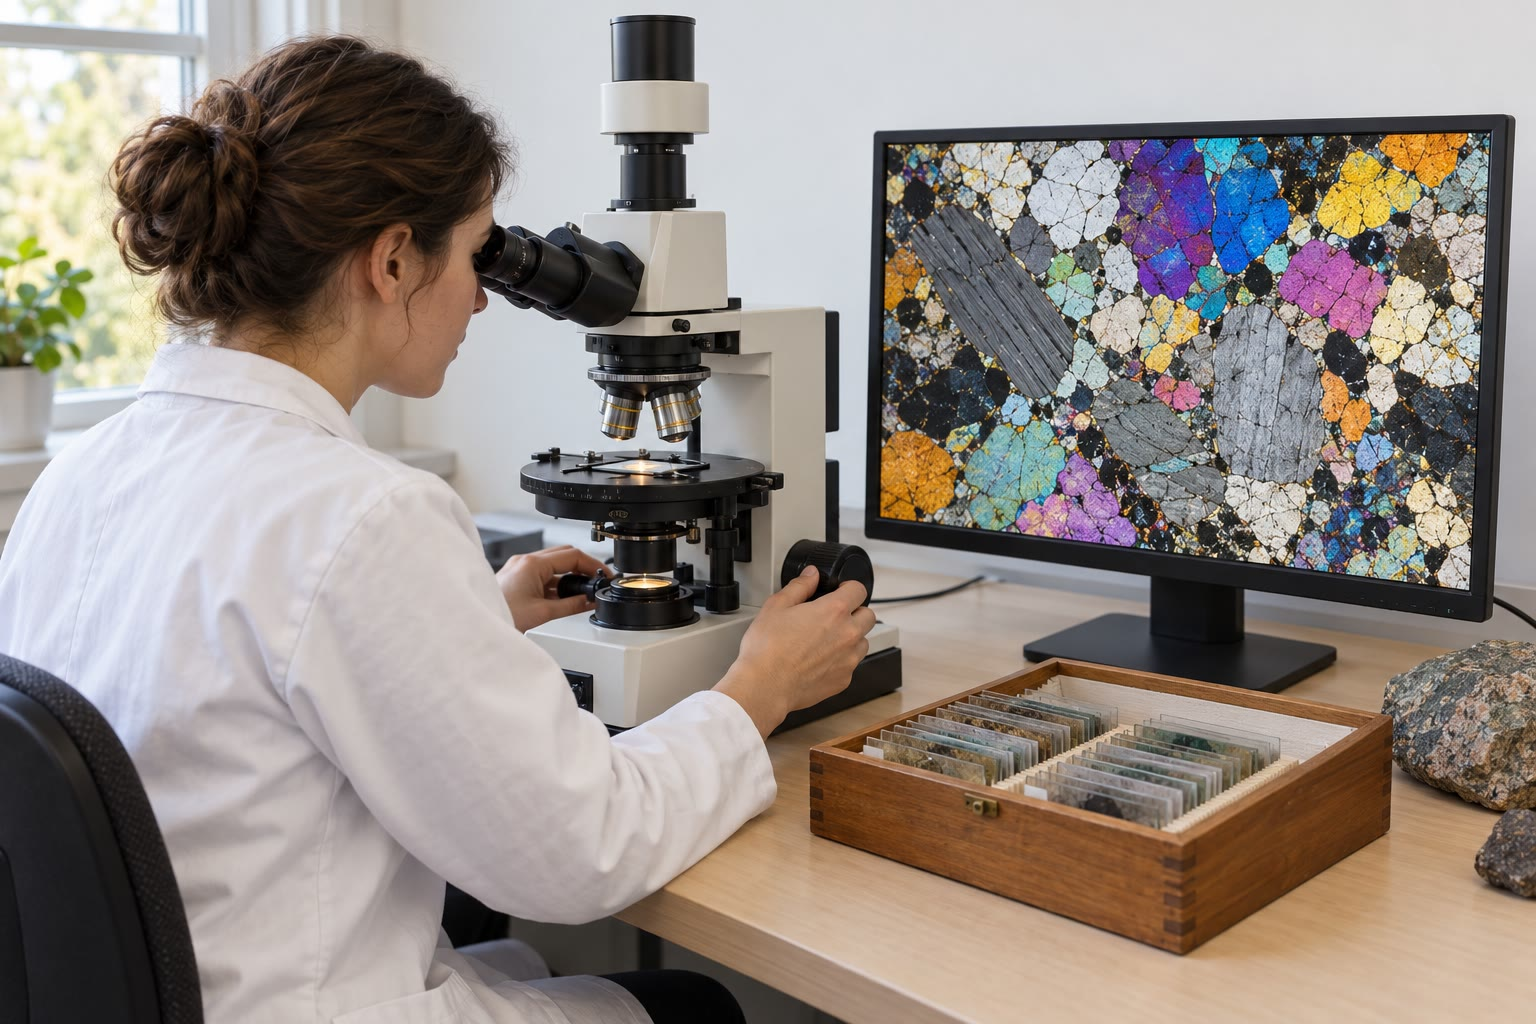
\includegraphics[width=\linewidth]{images/book5/ai/b3-petrology-desk.jpg}

{\scriptsize एक पेट्रोलॉजिस्ट ध्रुवण सूक्ष्मदर्शी पर, पास में पतली काटों का एक डिब्बा और स्क्रीन पर
ध्रुवित प्रकाश में एक पतली काट लिए हुए,
(AI से बनाया गया चित्रण)।}
\end{minipage}
\end{inthelab}

\section{अभ्यास}

\begin{exercise}[$\star$]\label{exo:b3:petrological-thermodynamics:1}
सारणियों से, एल्बाइट के लिए $\Delta_fH^\circ = \qty{-3935.0}{kJ}$, $S^\circ =
\qty{207.4}{J.K^{-1}}$, $V = \qty{100.07}{cm^3}$; जेडेआइट $-3029.3$, 133.5,
60.40; क्वार्ट्ज़ $-910.7$, 41.5, 22.69 (प्रति मोल)। एल्बाइट = जेडेआइट + क्वार्ट्ज़ के लिए,
$\Delta_rH$, $\Delta_rS$, $\Delta_rV$ (\unit{J.bar^{-1}} में), क्लेपेरॉन ढलान
और \qty{600}{\celsius} पर रेखा का दाब, स्थिर गुणधर्म मानकर
परिकलित कीजिए।
\end{exercise}
% ledger: rh95:ab-jd-qz

\begin{exercise}[$\star$]\label{exo:b3:petrological-thermodynamics:2}
\ce{MgO}--\ce{SiO2} तंत्र की एक चट्टान में फ़ोर्स्टेराइट, एन्स्टाटाइट और
क्वार्ट्ज़ मिलते हैं। \omterm{prop:b3:petrological-thermodynamics:goldschmidt}{खनिजीय प्रावस्था नियम} लागू कीजिए। आप क्या निष्कर्ष निकालते हैं?
\end{exercise}

\begin{exercise}[$\star$]\label{exo:b3:petrological-thermodynamics:3}
एक गार्नेट में, जिसमें
$X_{\text{Ca}} = 0.20$ और $X_{\text{Mg}} = 0.15$ है, ग्रॉसुलर और पायरोप की आदर्श सक्रियताएँ,
और एक प्लैजियोक्लेज़ में, जिसमें $X_{\text{ऐन}} = 0.40$ है, ऐनॉर्थाइट की (एक स्थल) सक्रियता परिकलित कीजिए।
\end{exercise}

\begin{exercise}[$\star$]\label{exo:b3:petrological-thermodynamics:4}
जिसमें $W =
\qty{15}{kJ.mol^{-1}}$ है, नियमित विलयन का क्रांतिक तापमान परिकलित कीजिए। कौन-सा $W$ $T_c = \qty{1000}{K}$ देता है?
\end{exercise}

\begin{exercise}[$\star\star$]\label{exo:b3:petrological-thermodynamics:5}
\qty{1000}{K} पर सारणियाँ निर्माण की गिब्स ऊर्जाएँ देती हैं,
$-5432.2$ (ग्रॉसुलर), $-3478.1$ (ऐनॉर्थाइट), $-2088.8$ (काइनाइट) और $-730.2$
(क्वार्ट्ज़), \unit{kJ.mol^{-1}} में। \qty{1}{bar} पर GASP अभिक्रिया का $\Delta_rG$ और
उसका साम्य दाब परिकलित कीजिए तथा प्रायोगिक
रेखा $P_0 = 22.80\,T - 1093$ (bar, \unit{\celsius}) से तुलना कीजिए।
\end{exercise}
% ledger: rh95:gasp-ht, kn88:gasp

\begin{exercise}[$\star\star$]\label{exo:b3:petrological-thermodynamics:6}
आकृति के नियमित विलयन ($W = \qty{20}{kJ.mol^{-1}}$) के लिए,
$G_{\text{मिश्र}}$ का मान $x = 0.5$ और \qty{900}{K} पर, फिर \omterm{def:b3:petrological-thermodynamics:solvus}{सॉल्वस} पार्श्व पर $x =
0.111$ पर परिकलित कीजिए। दिखाइए कि संघटन 0.5 वाले क्रिस्टल को दो पार्श्वों में बाँटने से
उसकी गिब्स ऊर्जा घटती है, और यह कितनी घटती है।
\end{exercise}

\begin{exercise}[$\star\star$]\label{exo:b3:petrological-thermodynamics:7}
तीन घटकों वाले तंत्र में एक निश्चर बिंदु पर कितनी प्रावस्थाएँ मिलती हैं, और कितनी
एकचरी रेखाएँ उससे निकलती हैं? आकृति के गुच्छे में
चारों अभिक्रियाओं में से प्रत्येक के संतुलित होने की जाँच कीजिए।
\end{exercise}

\begin{exercise}[$\star\star$]\label{exo:b3:petrological-thermodynamics:8}
आकृति के नियमित विलयन में स्थूल संघटन $X_0 = 0.3$ वाली एक चट्टान
\qty{900}{K} तक ठंडी हो चुकी है, जहाँ \omterm{def:b3:petrological-thermodynamics:solvus}{सॉल्वस} के पार्श्व 0.111 और 0.889 हैं।
प्रत्येक प्रावस्था का अनुपात परिकलित कीजिए।
\end{exercise}

\begin{exercise}[$\star\star$]\label{exo:b3:petrological-thermodynamics:9}
GASP भूदाबमापी $P = P_0 + (3RT/6.21)\ln(X_{\text{Ca}}/X_{\text{ऐन}})$ के साथ
(bar) में, \qty{900}{K} पर $\partial P/\partial X_{\text{ऐन}}$ का मान परिकलित कीजिए, जब
$X_{\text{ऐन}} = 0.30$ पर बताइए कि $X_{\text{ऐन}}$ में 0.01 की त्रुटि
दाब को कितना हिलाती है?
\end{exercise}

\begin{exercise}[$\star\star\star$]\label{exo:b3:petrological-thermodynamics:10}
दिखाइए कि नियमित विलयन का स्पिनोडल $x(1 - x) = RT/(2W)$ है। किस
तापमान पर संघटन 0.3 वाला क्रिस्टल किसी भी छोटे
उतार-चढ़ाव के प्रति अस्थिर हो जाता है, $W = \qty{20}{kJ.mol^{-1}}$ के लिए? उस तापमान की तुलना कीजिए
जिस पर वह \omterm{def:b3:petrological-thermodynamics:solvus}{सॉल्वस} तक पहुँचता है, $T = W(1 - 2x)/[R\ln((1 - x)/x)]$ के साथ, और
अंतर की व्याख्या कीजिए।
\end{exercise}

\begin{exercise}[$\star\star\star$]\label{exo:b3:petrological-thermodynamics:11}
दिखाइए कि सममित नियमित विलयन का \omterm{def:b3:petrological-thermodynamics:solvus}{सॉल्वस} $RT\ln[x/(1 -
x)] + W(1 - 2x) = 0$ को संतुष्ट करता है, और यह अपने अधिकतम मान $T_c = W/(2R)$ तक, $x
= 1/2$ पर पहुँचता है।
\end{exercise}

\begin{exercise}[$\star\star\star$]\label{exo:b3:petrological-thermodynamics:12}
एक चट्टान में \qty{2.0}{wt\percent} \ce{MnO} होता है। गार्नेट के क्रोड, जिनमें
\qty{10}{wt\percent} \ce{MnO} होता है, चट्टान का \qty{8}{wt\percent} भाग बनाते हैं और
मैट्रिक्स से पृथक रहते हैं। \omterm{def:b3:petrological-thermodynamics:pseudosection}{प्रभावी स्थूल संघटन} में \ce{MnO} की मात्रा
परिकलित कीजिए। गार्नेट के रिम के \omterm{def:b3:petrological-thermodynamics:pseudosection}{छद्मकाट} के लिए यह क्यों महत्वपूर्ण है?
\end{exercise}

\section{समस्या: वार्डन शिस्ट का गार्नेट}

\begin{problem}[{सप्ताहांत समस्या --- एक काल्पनिक शिस्ट का दाब और तापमान,
सारणियों, प्रावस्था नियम, सक्रियता मॉडल और
थर्मोबैरोमेट्री से}]
\label{pb:b3:petrological-thermodynamics:1}
% values: calc/ch11.py; gasp_tables.py
वार्डन पहाड़ियों के आधारशैल की शिस्ट, जो लगभग
\qty{480}{Ma} पहले कायांतरित हुई, उसमें गार्नेट, बायोटाइट, मस्कोवाइट, प्लैजियोक्लेज़, काएनाइट और
क्वार्ट्ज़ मिलते हैं। गार्नेट के रिम पर और उसके आसपास के कणों में माइक्रोप्रोब
से ये मान मिलते हैं: गार्नेट $X_{\text{Fe}} = 0.74$, $X_{\text{Mg}} = 0.12$, $X_{\text{Ca}} =
0.10$, $X_{\text{Mn}} = 0.04$; बायोटाइट $\ce{Mg}/(\ce{Mg} + \ce{Fe}) = 0.45$;
प्लैजियोक्लेज़ $X_{\text{ऐन}} = 0.30$। GASP अभिक्रिया के लिए इस अध्याय की सारणियाँ,
पुस्तक 4 (स्नातक वर्ष 2) का तापमापी
\[
T = \frac{52\,635 + 0.311P}{20.20 - 3R\ln K_D}\quad(T \text{ K में}, P
\text{ bar में}),
\]
और उसका प्रायोगिक दाबमापी $P = 22.80\,t - 1093 + (3RT/6.21)\ln
(X_{\text{Ca}}/X_{\text{ऐन}})$, जहाँ $t$ \unit{\celsius} में और $T$ केल्विन में हो, उपयोग कीजिए।
मान लीजिए $R = \qty{8.314}{J.mol^{-1}.K^{-1}}$ और भूपर्पटी का
घनत्व \qty{2800}{kg/m^3} तथा $g = \qty{9.81}{m/s^2}$ है।

\medskip\noindent\textbf{भाग I --- सारणियाँ।}
\begin{enumerate}
  \item सारांश सारणी से $\Delta_rH^\circ$, $\Delta_rS^\circ$
        तथा GASP अभिक्रिया का $\Delta_rV$ परिकलित कीजिए।
  \item \qty{298.15}{K} और \qty{1}{bar} पर $\Delta_rG$ परिकलित कीजिए। सतह पर
        कौन-सा पक्ष स्थायी है?
  \item गुणों को स्थिर मानते हुए \qty{900}{K} पर अंत्य-सदस्य दाब
        और क्लेपेरॉन ढलान परिकलित कीजिए।
  \item उच्च-तापमान सारणियाँ \qty{900}{K} पर $\Delta_rG = \qty{81.5}{kJ}$ और
        \qty{1200}{K} पर \qty{119.8}{kJ} देती हैं (\qty{1}{bar} पर)।
        दाब परिकलित कीजिए।
  \item उन्हीं तापमानों पर प्रयोगात्मक रेखा से तुलना कीजिए।
  \item $\Delta_rH$ में कौन-सी त्रुटि \qty{1200}{K} पर इस अंतर की व्याख्या कर सकती है?
        चारों एन्थैल्पियों की संयुक्त अनिश्चितता से तुलना कीजिए।
  \item ऊष्मा-धारिताएँ परिणाम को इतना कम क्यों बदलती हैं?
\end{enumerate}

\medskip\noindent\textbf{भाग II --- प्रावस्था नियम।}
\begin{enumerate}[resume]
  \item छह खनिजों और एक जल-तरल का वर्णन करने के लिए आवश्यक घटक सूचीबद्ध कीजिए
        और प्रावस्थाएँ गिनिए।
  \item प्रावस्था नियम से विचरण परिकलित कीजिए, और
        \omterm{prop:b3:petrological-thermodynamics:goldschmidt}{खनिजीय प्रावस्था नियम} की जाँच कीजिए।
  \item एक दूसरा नमूना काएनाइट और सिलिमेनाइट को साथ-साथ रखता है।
        इससे उसके दाब और तापमान के बारे में क्या पता चलता है?
  \item कायांतरण के दौरान चट्टान में से जल प्रवाहित हुआ। इससे
        गिनती कैसे बदलती है?
\end{enumerate}

\medskip\noindent\textbf{भाग III --- सक्रियताएँ और थर्मोबैरोमेट्री।}
\begin{enumerate}[resume]
  \item ग्रॉसुलर और एनॉर्थाइट की आदर्श सक्रियताएँ, तथा चट्टान में GASP अभिक्रिया का
        $\ln K$ परिकलित कीजिए।
  \item गार्नेट--बायोटाइट विनिमय का $K_D$ परिकलित कीजिए।
  \item \qty{8}{kbar} पर तापमान परिकलित कीजिए।
  \item उस तापमान पर GASP दाब परिकलित कीजिए।
  \item दोनों समीकरणों के प्रतिच्छेदन तक पुनरावृत्ति कीजिए।
  \item सारणियों की अंत्य-सदस्य रेखा के साथ, प्रायोगिक रेखा के स्थान पर, प्रतिच्छेदन
        पुनः ज्ञात कीजिए ($\Delta_rV = \qty{-6.61}{J.bar^{-1}}$ लेकर)।
        कौन-सा परिणाम आप रखेंगे, और क्यों?
  \item $X_{\text{ऐन}}$ में 0.05 की त्रुटि परिणाम को कितना
        खिसकाती है?
\end{enumerate}

\medskip\noindent\textbf{भाग IV --- दफ़न।}
\begin{enumerate}[resume]
  \item पुस्तक 4 (स्नातक वर्ष 2) के स्थिर गुणों के साथ, काएनाइट = सिलिमेनाइट
        अभिक्रिया के लिए $\Delta_rH = \qty{7.7}{kJ}$, $\Delta_rS =
        \qty{12.6}{J.K^{-1}}$, $\Delta_rV = \qty{0.571}{J.bar^{-1}}$। क्या
        परिणाम काएनाइट क्षेत्र में है?
  \item दफ़न की गहराई परिकलित कीजिए।
  \item गार्नेट क्रोड का $X_{\text{Ca}} = 0.07$ है, और वह लगभग उसी तापमान पर
        उसी $X_{\text{ऐन}}$ वाले प्लैजियोक्लेज़ के साथ बढ़ा। क्या क्रोड
        रिम की तुलना में अधिक गहराई पर या कम गहराई पर बना?
  \item वार्डन शिस्ट का शिखर दाब और दफ़न की गहराई बताइए।
\end{enumerate}
\end{problem}
